% Compile: pdflatex main && bibtex main && pdflatex main && pdflatex main
\documentclass{article}

% Official NeurIPS 2026 workshop style (anonymous / double-blind).
\usepackage[dblblindworkshop]{neurips_2026}
\workshoptitle{Symmetry and Geometry in Neural Representations (NeurReps)}

\usepackage[utf8]{inputenc}
\usepackage[T1]{fontenc}
\usepackage{amsmath,amssymb,amsfonts}
\usepackage{booktabs}
\usepackage{graphicx}
\usepackage{placeins}
\usepackage{url}
\usepackage{microtype}
\usepackage{xcolor}

\title{Native Geometry vs.\ Linear Recoverability:\\
Testing Platonic Scaling Across Astronomical Surveys}

\author{Anonymous Author(s)}

\usepackage{hyperref}
\begin{document}

\maketitle

\begin{abstract}
The Platonic Representation Hypothesis predicts increasing representational convergence with model scale, but convergence depends on the transformation class under which representations are compared.
Across matched Legacy Survey and HSC embeddings from five model families, supervised linear alignment steepens the model-size dependence of cross-survey neighbourhood correspondence relative to native cosine geometry.
The amplification occurs in all five families and persists at fixed rank \(256\), ruling out increased alignment dimensionality from wider embeddings as the explanation.
The fitted maps remain broadly anisotropic, while most of their mKNN gain is carried by a small singular subspace.
Sparse SAE and BSF representations provide no advantage over the matched dense-alignment baseline.
Thus scaling strengthens linear recoverability more clearly than native geometric similarity.
\end{abstract}

\section{Introduction}\label{sec:intro}

Representations from independently trained models often become more aligned as capability and scale increase~\citep{huh2024platonic}.
The Platonic Representation Hypothesis (PRH) interprets this as convergence toward a shared statistical model of reality.
Matched Legacy Survey~\citep{dey2019legacy}\(\leftrightarrow\)HSC~\citep{miyazaki2018hsc} embeddings provide a comparatively clean testbed: prior work reports increasing mutual \(k\)-nearest-neighbour (mKNN) agreement with model capacity~\citep{duraphe2025platonicuniverse}.
The central question is not whether any cross-survey signal exists, but whether its \emph{strength} depends on the transformation class under which equivalence is assessed.

A substantial literature studies how to \emph{align} independently trained embedding spaces: geometry-preserving orthogonal/Procrustes registration~\citep{mikolov2013exploiting}, supervised linear interoperability between representations, and unpaired or pseudo-paired embedding translation~\citep{lample2018word,moschella2023relative,jha2025vec2vec}.
Our contribution is not that linear maps can align embeddings.
Rather, we ask how the apparent \emph{scaling} of representational convergence changes with the permitted transformation class, and whether the maps that improve recoverability are themselves becoming geometrically simpler.

We organize allowed maps as
\(\mathcal{T}_{\mathrm{id}}\subset\mathcal{T}_{\mathrm{scaled\,orth}}\subset\mathcal{T}_{\mathrm{affine}}\).
At \(\mathcal{T}_{\mathrm{id}}\), representations are compared in native coordinates.
At \(\mathcal{T}_{\mathrm{scaled\,orth}}\), equivalence is assessed up to rotation/reflection and global scaling (\(x\mapsto cQx\) with \(Q^\top Q=I\)); such maps preserve all pairwise cosines and therefore cosine \(k\)NN structure.
At \(\mathcal{T}_{\mathrm{affine}}\), supervised Ridge may apply anisotropic linear deformation plus translation.
Under the primary cosine-mKNN observable, identity and scaled-orthogonal reparameterizations are observationally indistinguishable, since \(\cos(cQx_i,cQx_j)=\cos(x_i,x_j)\) for \(c>0\).
The experimentally meaningful comparison is therefore native cosine geometry (modulo scaled-orthogonal transforms) versus supervised affine-linear recoverability.

On the same held-out objects we measure \emph{native correspondence}
\(M_{\mathrm{native}}\equiv M_{\mathrm{Dense}}\) (raw cosine mKNN) and \emph{linear recoverability}
\(M_{\mathrm{linear}}\equiv M_{\mathrm{Dense+Ridge}}\) (mKNN after a supervised global Ridge map fit on paired training objects).
The \emph{alignment gain} is \(G=M_{\mathrm{linear}}-M_{\mathrm{native}}\).
We use ``linear recoverability'' as shorthand for correspondence exposed by this affine predictor's linear component (Section~\ref{sec:setup}).

We report three claims.
\textbf{(1)}~Linear recoverability scales more strongly with model size than native correspondence.
\textbf{(2)}~This survives fixed independent-PCA rank \(256\), so it cannot be explained simply by larger models giving Ridge a higher-dimensional map.
\textbf{(3)}~The fitted linear components remain broadly anisotropic, yet most of their mKNN lift is carried by a comparatively small singular subspace.
Secondary controls---PCA bottlenecks, sparse SAE~\citep{gao2025sae}/BSF~\citep{fel2026bsf} representations, a same-dataset cross-model symmetry check, and an unpaired nonlinear bottleneck---are reported in the appendix.

\section{Setup}\label{sec:setup}

We use the official UniverseTBD Legacy\(\leftrightarrow\)HSC matched embeddings~\citep{duraphe2025platonicuniverse} (\(n{=}16{,}384\) objects) across five families---AstroPTv2~\citep{smith2024astropt}, ConvNeXtv2~\citep{woo2023convnextv2}, DINOv2~\citep{oquab2024dinov2}, ViT~\citep{dosovitskiy2021vit}, and I-JEPA~\citep{assran2023ijepa}---sixteen size rungs in total (Appendix~\ref{app:details}).
I-JEPA has only two rungs.

For representations \(A\) and \(B\),
\[
M_k=\frac{1}{n}\sum_i
\frac{\lvert \mathcal N_k^A(i)\cap \mathcal N_k^B(i)\rvert}{k},
\]
with cosine neighbours and self-exclusion~\citep{huh2024platonic,duraphe2025platonicuniverse}.
The primary scale is \(k{=}10\).
All primary results use a frozen train/test split (\(n_{\mathrm{train}}{=}13{,}107\), \(n_{\mathrm{test}}{=}3277\), seed \(0\)) and a \textbf{test-only gallery}: neighbours are sought among held-out objects only (chance \(\approx 0.0031\)).
Direction is Legacy\(\to\)HSC\@.
We fit an affine Ridge predictor after train-only standardization (\(\mathrm{StandardScaler}\) on \(X,Y\), then Ridge with \(\alpha{=}1\) and an intercept).
Because our geometric diagnostics characterize its linear component \(A_{\mathrm{eff}}\) in original coordinates, we use ``linear recoverability'' as shorthand for correspondence exposed by this affine-linear alignment (Appendix~\ref{app:geometry}).

\section{Linear recoverability scales more strongly than native correspondence}\label{sec:scaling}

Supervised linear alignment raises both the level and the model-size slope of cross-survey correspondence.
Mean held-out mKNN@10 is \(0.022\) for native correspondence and \(0.042\) for linear recoverability (alignment gain \(G\approx0.020\); Figure~\ref{fig:scaling}a)---roughly a doubling of native overlap and \(\sim\!13\times\) chance (\(\approx0.0031\)), without claiming downstream astrophysical utility.
Family OLS slopes of mKNN versus \(\log_{10}P\) steepen under Ridge:
\[
\Delta\beta_F=\beta_{\mathrm{Dense+Ridge},F}-\beta_{\mathrm{Dense},F}
\]
is positive in all five families, giving
\[
T=\frac15\sum_F\Delta\beta_F=0.00721.
\]
We average family slope differences equally so that the architecture family---not the number of published checkpoints within a family---is the unit of replication (Appendix~\ref{app:stats}).
The amplification is positive in all five architecture families (\(p_{\mathrm{sign}}{=}0.031\)), remains positive under held-out-object bootstrap (95\% CI \([0.0034,0.0111]\)), and exceeds a synchronized correspondence-shuffle refit null (\(p_{\mathrm{perm}}\approx0.005\); Appendix~\ref{app:stats}).
It remains positive across neighbourhood sizes \(k\in\{5,10,25,50\}\); the reverse HSC\(\to\)Legacy map also yields \(T_{H\to L}>0\), though with smaller magnitude and one negative family (Appendix~\ref{app:dirk}).

The same pattern survives at fixed representation dimension.
Using \emph{independent} survey PCAs at rank \(r{=}256\) (Appendix~\ref{app:pca}), native \(M_{\mathrm{indPCA256}}\) and supervised \(M_{\mathrm{indPCA256+Ridge}}\) share the same 256-dimensional features.
Defining
\[
\Delta\beta_{F,256}
=\beta_{\mathrm{indPCA256+Ridge},F}-\beta_{\mathrm{indPCA256},F},
\qquad
T_{256}=\frac15\sum_F\Delta\beta_{F,256}=0.00864,
\]
we find \(\Delta\beta_{F,256}>0\) in all five families (\(T_{256}^{(-I)}=0.00673\) excluding I-JEPA).
The effect persists when alignment is restricted to the same 256-dimensional representation space, so it cannot be explained simply by larger models giving Ridge a higher-dimensional map (Figure~\ref{fig:scaling}b).

\begin{figure}[t]
\centering
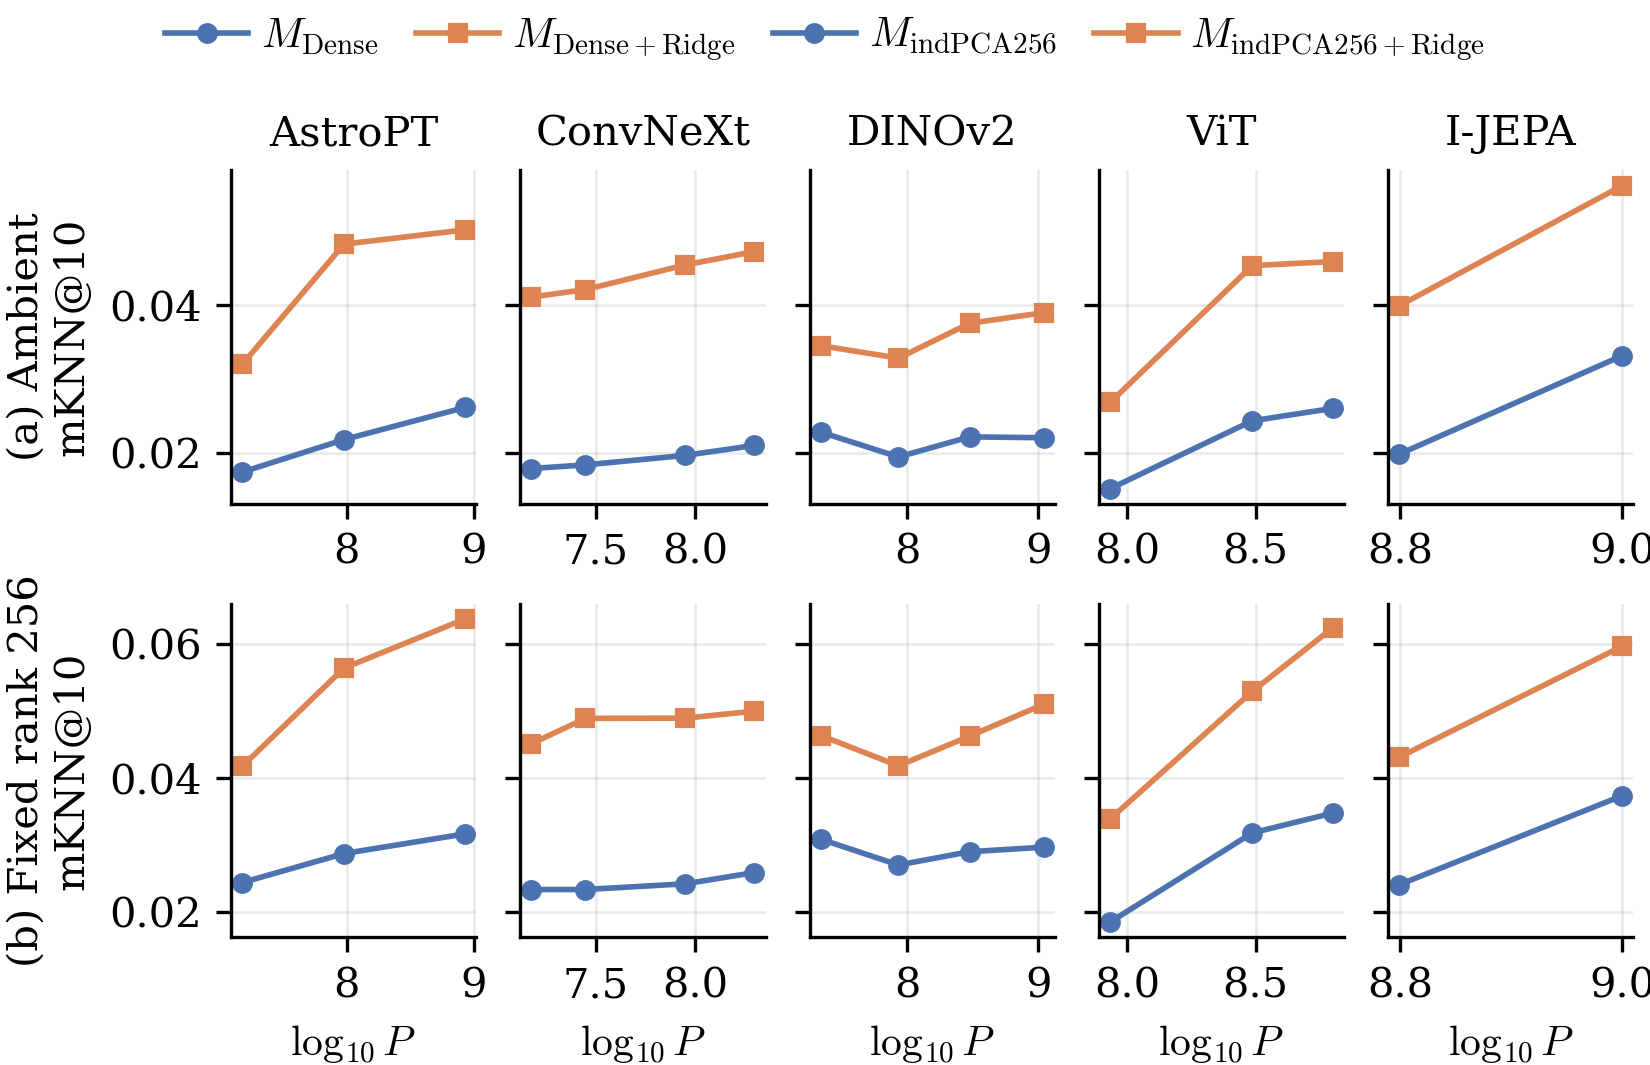
\includegraphics[width=\linewidth]{figures/scaling_dense_and_fixedrank.png}
\caption{\textbf{(a)}~Held-out mKNN@10 versus \(\log_{10}P\): native \(M_{\mathrm{native}}\) vs.\ linear \(M_{\mathrm{linear}}\).
\textbf{(b)}~Fixed independent-PCA rank \(256\). Supervised alignment steepens scaling in both settings (\(T{>}0\), \(T_{256}{>}0\)).}\label{fig:scaling}
\end{figure}

\section{Recoverability is concentrated within broadly anisotropic maps}\label{sec:geometry}

Because scaled-orthogonal maps \(x\mapsto cQx\) preserve pairwise cosine similarities, they cannot change cosine mKNN; the observed gain must depend on deformation outside this class (and, for the full affine map, potentially translation).
We characterize the learned linear component
\(A_{\mathrm{eff}}=\mathrm{diag}(\sigma_y)W\mathrm{diag}(1/\sigma_x)\)
in original coordinates (\(W{=}\)Ridge \(\texttt{coef\_}\); Appendix~\ref{app:geometry}).

Writing \(A_{\mathrm{eff}}=U\Sigma V^\top\), the log-singular-value dispersion
\(A_{\log}=\mathrm{std}_i(\log\sigma_i)\)
is \(1.76\)--\(3.15\) across rungs, so alignment requires substantial direction-dependent stretch rather than rotation/reflection and global rescaling alone.
Defining centered log-stretches \(a_i=\log\sigma_i-\tfrac1d\sum_j\log\sigma_j\) and anisotropy masses \(a_i^2\), let \(f_{90}^{\mathrm{anis}}\) be the fraction of singular directions required for \(90\%\) of \(\sum a_i^2\).
Across the \(16\) maps, \(f_{90}^{\mathrm{anis}}\) is \(0.411\)--\(0.490\) (median \(0.427\)):
departure from uniform scaling is spread across a substantial fraction of the representation.

\begin{figure}[!t]
\centering
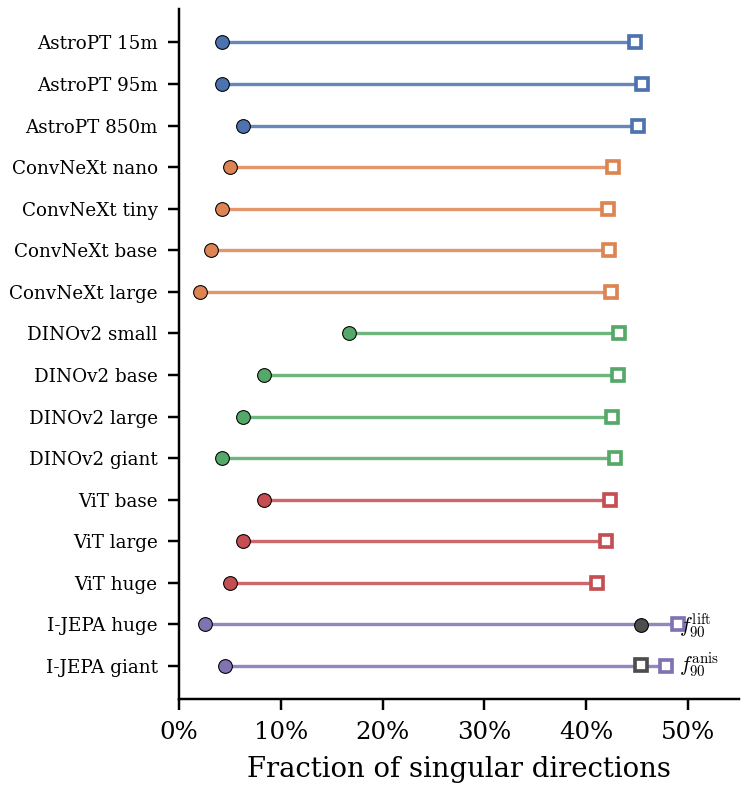
\includegraphics[width=0.72\linewidth,height=0.42\textheight,keepaspectratio]{figures/geometry_anisotropy_vs_functional.png}
\caption{Fraction of singular directions needed for \(90\%\) of Dense+Ridge mKNN lift (\(f_{90}^{\mathrm{lift}}\); filled) versus \(90\%\) of anisotropy mass (\(f_{90}^{\mathrm{anis}}\); open).
Medians \(4.8\%\) vs.\ \(42.7\%\); properties of the fitted map, not intrinsic rank.}\label{fig:geometry_concentration}
\end{figure}

Yet the deformation relevant to neighbourhood recovery is much more concentrated.
Truncating \(A_{\mathrm{eff}}\) along singular directions without refitting recovers \(90\%\) of the Dense+Ridge mKNN lift
\(G=M_{\mathrm{Dense+Ridge}}-M_{\mathrm{native}}\)
using only \(2.1\)--\(17\%\) of directions (median \(4.8\%\); Figure~\ref{fig:geometry_concentration}).
Spectral anisotropy and functional recoverability therefore have sharply different effective dimensionalities.

This contrast does not itself show a compelling size trend:
\(f_{90}^{\mathrm{anis}}\) decreases slightly in four of five families, but changes are only a few percentage points and the pooled association with \(\log_{10}P\) is weak
(descriptive Spearman \(\rho{=}0.13\), \(p{=}0.64\), \(n{=}16\));
\(A_{\log}\) and \(f_{90}^{\mathrm{anis}}\) are likewise weakly associated (\(\rho{=}0.39\), \(p{=}0.13\); Appendix~\ref{app:geometry}).
Scaling therefore strengthens linear recoverability without corresponding simplification of the native metric geometry, while the part of \(A_{\mathrm{eff}}\) that matters for cosine-neighbour recovery remains functionally low-dimensional.

\section{Discussion and conclusion}\label{sec:disc}

Apparent representational convergence depends on the permitted transformation class.
Native cosine correspondence grows only weakly with model size, and scaled-orthogonal maps leave cosine neighbourhoods unchanged.
At \(\mathcal{T}_{\mathrm{affine}}\), supervised recoverability is clearly amplified (\(T{=}0.00721\); \(5/5\)) and survives fixed independent-PCA dimension (\(T_{256}{=}0.00864\); \(5/5\)).
Translation ablation leaves most absolute gain and slope amplification intact, so the effect is primarily carried by anisotropic \(A_{\mathrm{eff}}\) (Appendix~\ref{app:geometry}).
The geometry of the fitted maps further separates native similarity from recoverability: although the effective linear transformations are broadly anisotropic---a median \(43\%\) of singular directions account for \(90\%\) of their departure from uniform scaling---their contribution to neighbourhood recovery is much more concentrated (median \(4.8\%\) of directions recovers \(90\%\) of the Dense+Ridge mKNN lift).
Thus linear recoverability can be functionally low-dimensional even when the alignment map as a whole is not a low-dimensional deformation.
Reverse amplification is weaker (\(T_{H\to L}{=}0.00447\)); a same-observation control retains \(R_{A\to B}\neq R_{B\to A}\) (Appendix~\ref{app:dirk},\ref{app:crossmodel}).
Limitations: paired Ridge supervision, five families, one astronomy setting, frozen split; \(T\) is stable across Ridge \(\alpha\) and \(k\) (Appendix~\ref{app:stats},\ref{app:dirk}).
Scaling strengthens supervised linear recoverability more clearly than native cosine similarity.

\FloatBarrier
{\small
\bibliographystyle{plainnat}
\bibliography{references}
}


\appendix
\section{Protocol and statistical robustness}\label{app:details}\label{app:stats}

Approximate parameter counts (\(10^{6}\)):
AstroPTv2 \(15/95/850\);
ConvNeXtv2 nano/tiny/base/large \(15/28/89/198\);
DINOv2 small/base/large/giant \(22/86/300/1100\);
ViT base/large/huge \(86/307/632\);
I-JEPA huge/giant \(630/1000\).

The primary statistic \(T=\tfrac15\sum_F\Delta\beta_F\) averages family slope differences equally so that architecture family---not checkpoint count---is the replication unit.
The forward effect is positive in all five families (\(p_{\mathrm{sign}}{=}0.03125\)), exceeds a synchronized correspondence-shuffle refit null (\(B{=}200\), \(p{=}1/201\approx0.005\)), and remains positive under held-out-object bootstrap (95\% CI \([0.0034,0.0111]\)); excluding I-JEPA gives \(T_{-I}{=}0.00537\) with four/four families positive.
The result is also stable across \(\alpha\in\{0.01,0.1,1,10,100\}\), with \(T(\alpha)\in[0.00721,0.00848]\) and \(5/5\) positive families throughout.

\section{Direction and neighbourhood-size robustness}\label{app:dirk}

All checks reuse the frozen train/test split, Ridge recipe, and test-only gallery.

\paragraph{Reverse direction.}
HSC\(\to\)Legacy yields \(T_{H\to L}{=}0.00447\) with \(4/5\) families positive (AstroPT negative).
Excluding I-JEPA, \(T_{H\to L}^{(-I)}{=}0.00103\).
Reverse amplification is present but weaker and family-heterogeneous; it is not a second primary claim.

\paragraph{Neighbourhood size.}
Aggregate forward amplification is stable across \(k\in\{5,10,25,50\}\):
\(T(k)\in\{0.00782,0.00721,0.00810,0.00869\}\),
with \(5/5\) positive families at \(k{=}5,10\) and \(4/5\) at \(k{=}25,50\).

\paragraph{Pooled interaction.}
On a rung\(\times\)method table, a family-fixed-effects OLS specification
\(M=\alpha_F+\gamma_F\log_{10}P+\delta_F R+\theta(R\log_{10}P)\)
gives the same positive interaction direction (\(\theta{=}0.00451\)), providing a descriptive robustness check under a different weighting.
We do not treat ordinary IID OLS uncertainties for this pooled model as primary inference, because Dense/Ridge observations are paired by rung.
Equal-family \(T\), the family sign test, the synchronized shuffle-refit null, and the object bootstrap remain the primary evidence.

\section{Secondary representation controls}\label{app:pca}\label{app:fixedrank}\label{app:sparse}\label{app:residual}

\emph{Independent} PCA+Ridge raises absolute recoverability at mid/high ranks (means \(\approx0.044/0.050/0.055\) at \(128/256/512\)); the fixed-rank \(256\) result is reported in the main text.
A pooled train-only PCA basis without pairing leaves native mKNN near Dense (\(\approx0.024\) at rank \(256\)), showing that dimensional reduction alone does not substantially increase native correspondence.
PCA does not yield a consistent additional scale interaction beyond Dense+Ridge.

Under matched Ridge supervision, SAE and BSF underperform Dense+Ridge by \(0.0085\) and \(0.0062\) mKNN on average, respectively; family-bootstrap 95\% CIs are \([-0.0120,-0.0043]\) and \([-0.0104,-0.0007]\).
Sparse coding therefore provides no additional cross-survey correspondence once alignment supervision is controlled.
SAE protocol: width \(F{=}2048\), seed \(0\), TopK from available checkpoints, train-only Ridge/IDF, fixed Legacy\(\to\)HSC~\citep{gao2025sae}; BSF uses Vanilla signed codes with the same Ridge recipe~\citep{fel2026bsf}.
Inference-time TopK sensitivity is reported in Appendix~\ref{app:sae_topk}.

Global Ridge residuals remain weakly locally structured in source space (\(k\in\{10,25,50\}\); all \(16\times 3\) residual-permutation tests give \(p{=}1/201\)), but absolute residual cosine similarity is \(\approx0.01\) and mean relative held-out MSE reduction from a patch intercept is \(\ll0.1\%\); we do not fit local maps.

\section{SAE TopK sensitivity}\label{app:sae_topk}

Trained checkpoints use heterogeneous TopK in \(18\)--\(23\) with no common training-time \(K\) across all \(16\) rungs.
To test whether the sparse-control result depends on sparsity level, we therefore repeat the frozen Legacy\(\to\)HSC protocol under \emph{inference-time} TopK overrides \(K\in\{10,20,40\}\) on the preferred \(F{=}2048\) seed-\(0\) checkpoints, holding dictionary width, split, Ridge fitting, mapping direction, IDF, and the test-only gallery fixed.
Across this range the mean residual \(M_{\mathrm{SAE+Ridge}}-M_{\mathrm{Dense+Ridge}}\) stays negative (\(-0.0159\), \(-0.0085\), \(-0.0077\)), family-bootstrap 95\% CIs exclude zero, and the equal-family scaling interaction \(T_{\mathrm{SAE},K}\) remains non-positive (\(-0.0133\), \(-0.0099\), \(-0.0079\); at most one family positive).
Thus the sparse result is not specific to the original TopK choice: across the tested inference sparsity range, SAE does not improve correspondence over the matched Dense+Ridge baseline and does not yield a consistently stronger size trend (Figure~\ref{fig:sae_topk}).

\begin{figure}[t]
\centering
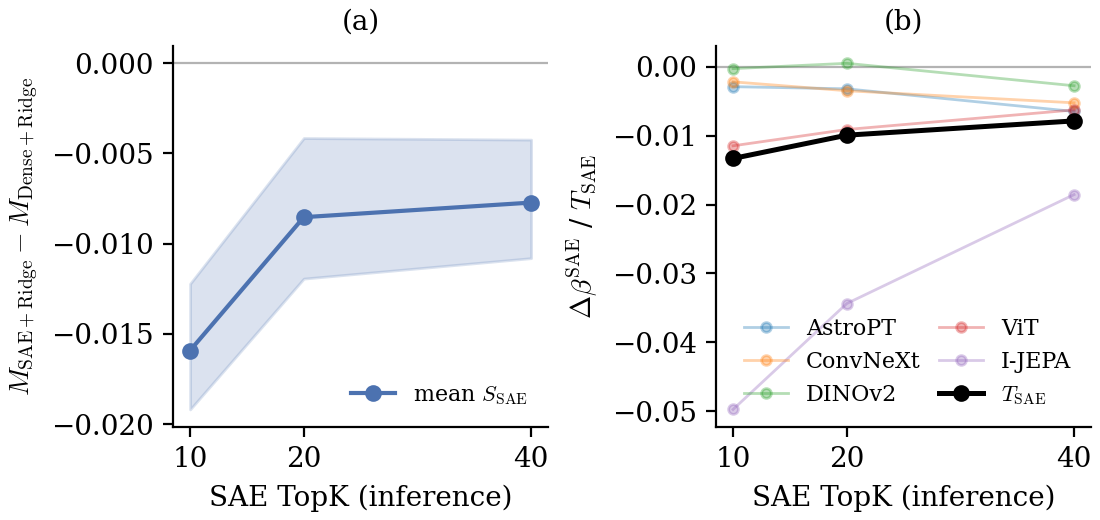
\includegraphics[width=\linewidth]{figures/sae_topk_sensitivity.png}
\caption{\textbf{(a)}~Mean SAE residual versus Dense+Ridge under inference-time TopK \(K\in\{10,20,40\}\) (family-bootstrap 95\% CI).
\textbf{(b)}~Equal-family scaling interaction \(T_{\mathrm{SAE},K}\) with per-family \(\Delta\beta^{\mathrm{SAE}}_{F,K}\) (faint).
Both absolute level and size interaction remain non-positive across \(K\).}\label{fig:sae_topk}
\end{figure}

\section{Geometry details}\label{app:geometry}

After train-only \(\mathrm{StandardScaler}\), Ridge yields \(W\) and an intercept in standardized coordinates.
The full affine map in original coordinates is \(\hat y=A_{\mathrm{eff}}x+b_{\mathrm{eff}}\) with
\(A_{\mathrm{eff}}=\mathrm{diag}(\sigma_y)W\mathrm{diag}(1/\sigma_x)\) and
\(b_{\mathrm{eff}}=\mu_y-A_{\mathrm{eff}}\mu_x+D_y b_{\mathrm{std}}\).
All spectral diagnostics below characterize the \emph{linear component} \(A_{\mathrm{eff}}\), not \(b_{\mathrm{eff}}\).

Writing \(A_{\mathrm{eff}}=U\Sigma V^\top\), we distinguish several quantities.
\emph{Magnitude of anisotropy.}
\(A_{\log}=\mathrm{std}_i(\log\sigma_i)\) measures overall departure from uniform scaling (\(1.76\)--\(3.15\) across rungs).
\emph{Concentration of anisotropy.}
Centered log-stretches \(a_i=\log\sigma_i-\mathrm{mean}_j\log\sigma_j\) yield anisotropy masses \(m_i=a_i^2\);
\(f_{90}^{\mathrm{anis}}\) is the fraction of singular directions required for \(90\%\) of \(\sum m_i\)
(\(0.411\)--\(0.490\); median \(0.427\)).
\emph{Functional concentration of lift.}
Truncating \(A_{\mathrm{eff}}\) along singular directions \emph{without refitting}, on the same held-out objects and test-only gallery, and defining
\(G_r=M_r-M_{\mathrm{native}}\) relative to the full-map lift \(G_{\mathrm{full}}\),
the smallest evaluated rank with \(G_r/G_{\mathrm{full}}\ge0.9\) uses
\(2.1\)--\(17\%\) of directions (median \(4.8\%\)).
Anisotropy concentration and functional lift concentration are therefore distinct measurements of the fitted map.
\emph{Distance from the cosine-preserving class.}
\(D_{\mathrm{sim}}=\min_{c,Q^\top Q=I}\|A_{\mathrm{eff}}-cQ\|_F/\|A_{\mathrm{eff}}\|_F\) is \(0.891\)--\(1.000\);
because scaled-orthogonal maps cannot change cosine mKNN, a large \(D_{\mathrm{sim}}\) characterizes the type of deformation required rather than independently explaining the gain.
\emph{Local stretch.}
On Legacy test \(k_{\mathrm{edge}}\)-NN edges \(\delta_{ij}\),
\(s_{ij}=\log(\|A_{\mathrm{eff}}\delta_{ij}\|_2/\|\delta_{ij}\|_2)\) with \(\sigma_{\mathrm{local}}=\mathrm{std}(s_{ij})\)
is \(0.157\)--\(0.310\) (\(k_{\mathrm{edge}}{=}10\)), so anisotropy also affects locally occupied held-out directions; \(\sigma_{\mathrm{local}}\) decreases with size in four of five families (suggestive, not conclusive).
Secondary spectral-energy diagnostics (\(H_{\mathrm{norm}}\)) likewise show non-flat maps.
Scale trends of \(A_{\log}\), \(f_{90}^{\mathrm{anis}}\), and \(\sigma_{\mathrm{local}}\) are shown in Figure~\ref{fig:geometry_scale};
pooled Spearman associations with \(\log_{10}P\) are weak for \(f_{90}^{\mathrm{anis}}\) (\(\rho{=}0.13\), \(p{=}0.64\)).

Because cosine mKNN is not translation-invariant, we ablate \(b_{\mathrm{eff}}\) without refitting: for each rung we compare native \(M(X,Y)\), full affine \(M(A_{\mathrm{eff}}X+b_{\mathrm{eff}},Y)\), and linear-only \(M(A_{\mathrm{eff}}X,Y)\) on the same test queries/gallery.
Affine reconstruction matches the sklearn pipeline to \(\max|{\rm err}|\le 3.5{\times}10^{-5}\).
Across the \(16\) rungs the fraction of affine gain retained by the linear component is \(\eta_A=\mathrm{median}\,0.990\) (mean \(0.985\); range \([0.920,1.048]\)).
Family slope amplification without translation is \(T_A{=}0.00854\) (\(5/5\) positive) versus \(T_{\mathrm{affine}}{=}0.00721\), so \(T_A/T_{\mathrm{affine}}{=}1.184\) (excluding I-JEPA, \(T_A^{(-I)}{=}0.00570\)).
A train-mean-centered diagnostic likewise preserves amplification (\(T_{\mathrm{centered}}{=}0.01360\); Figure~\ref{fig:translation_ablation}).
Thus the headline scaling effect is primarily attributable to anisotropic linear deformation rather than affine translation.

\begin{figure}[t]
\centering
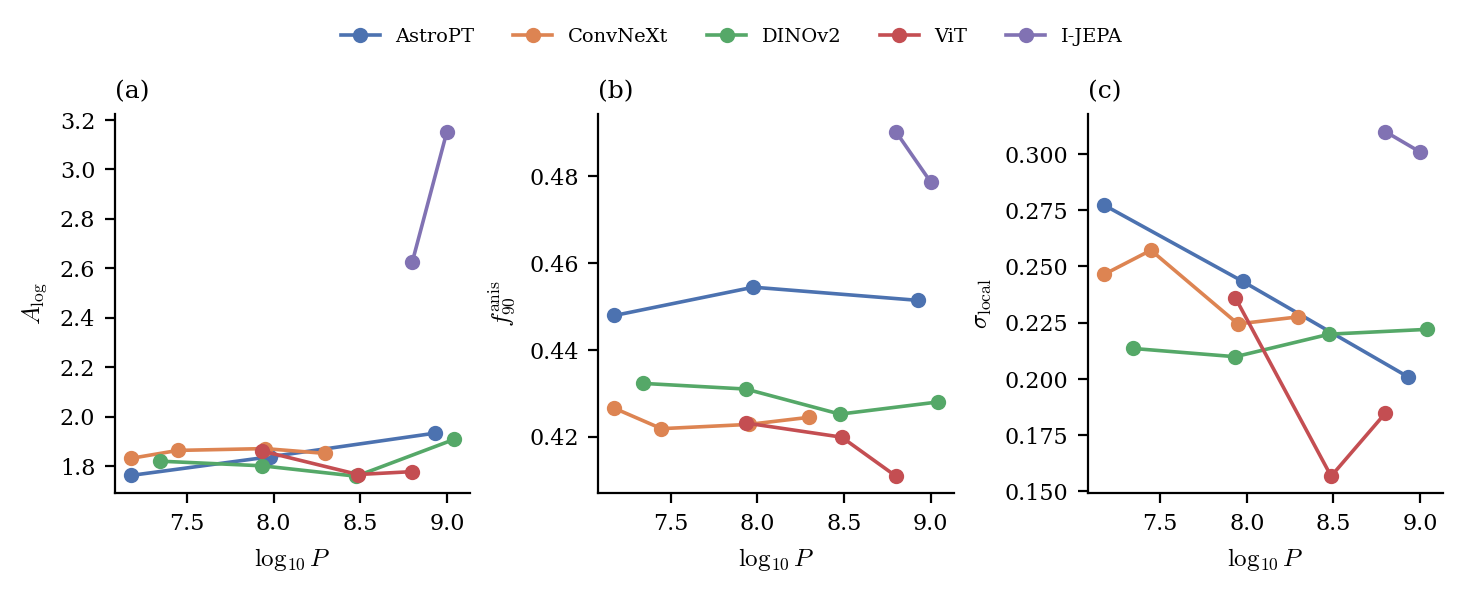
\includegraphics[width=\linewidth]{figures/geometry_scale_diagnostics.png}
\caption{Within-family trends versus \(\log_{10}P\):
\textbf{(a)}~anisotropy magnitude \(A_{\log}\);
\textbf{(b)}~anisotropy concentration \(f_{90}^{\mathrm{anis}}\);
\textbf{(c)}~local stretch dispersion \(\sigma_{\mathrm{local}}\) on held-out Legacy edges.
Points are connected only within architecture families.}\label{fig:geometry_scale}
\end{figure}

\begin{figure}[t]
\centering
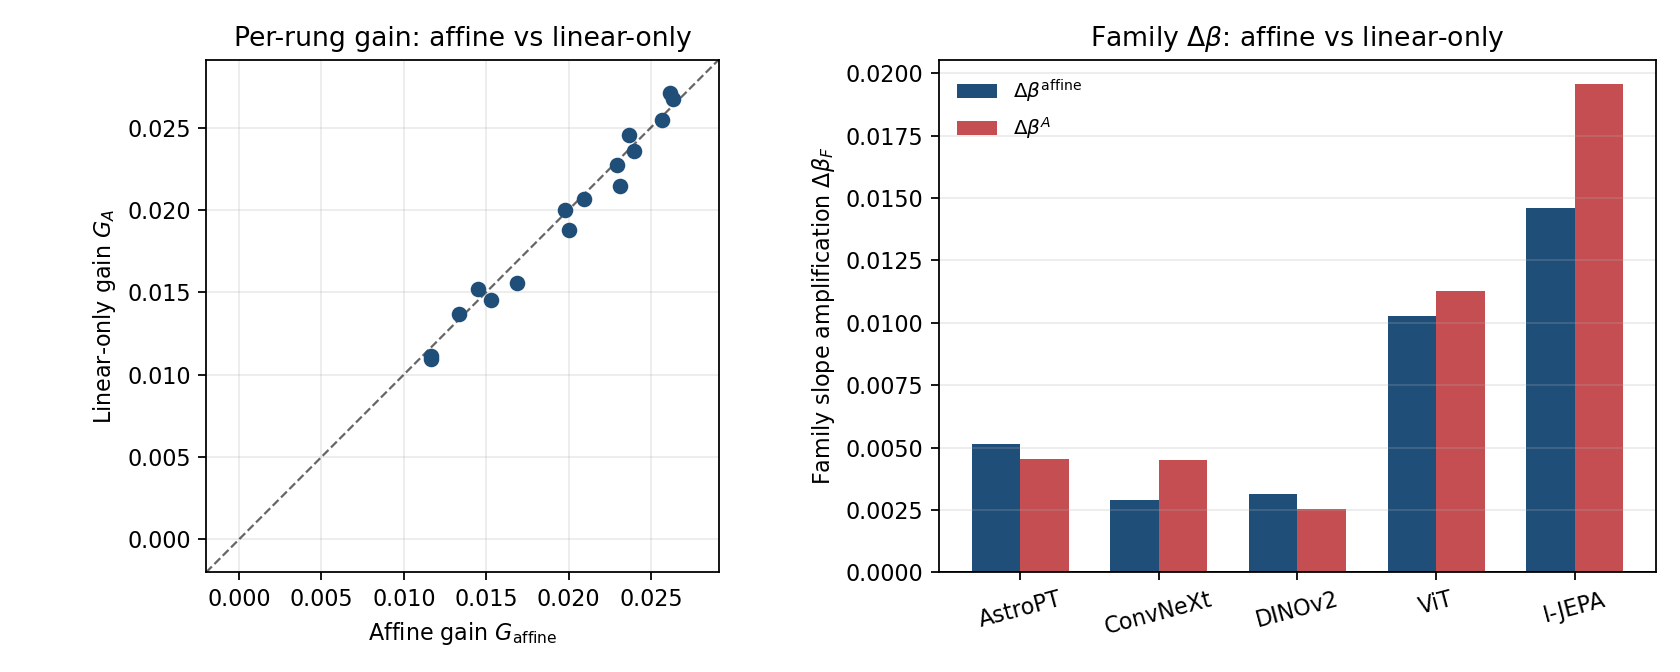
\includegraphics[width=\linewidth]{figures/translation_ablation_summary.png}
\caption{\textbf{(a)}~Per-rung Dense+Ridge mKNN gain with the full affine map versus the linear component alone (\(y{=}x\) dashed).
\textbf{(b)}~Family slope amplifications \(\Delta\beta_F\) for affine and linear-only conditions.
Removing \(b_{\mathrm{eff}}\) retains essentially all absolute gain and the model-size amplification.}\label{fig:translation_ablation}
\end{figure}

\section{Same-dataset cross-model control}\label{app:crossmodel}

Cross-survey directionality may reflect survey-information differences, so same-Legacy cross-model alignment tests whether asymmetry persists when the observation channel is fixed.
We evaluate all \(101\) valid unordered cross-family pairs among \(16\) Legacy models (train-only independent PCA256 per model; Ridge \(\alpha{=}1\); mKNN@10; test-only gallery; frozen 80/20 split; both directions fit independently).
For unordered pair \(\{A,B\}\),
\[
G_{\mathrm{sym}}=\tfrac12(G_{A\to B}+G_{B\to A}),
\qquad
A_{\mathrm{dir}}=|G_{A\to B}-G_{B\to A}|,
\]
where \(G_{A\to B}=M^{\mathrm{Ridge}}_{A\to B}-M_{\mathrm{native}}(A,B)\) and likewise for \(G_{B\to A}\).

Mean native mKNN is \(0.050\) (chance \(\approx0.00305\)).
Ridge increases correspondence in both directions for \(101/101\) pairs (mean \(G_{\mathrm{sym}}{=}0.060\); mean \(A_{\mathrm{dir}}{=}0.036\); mean relative asymmetry \(A_{\mathrm{rel}}{\approx}0.33\)).
Mean directional gain is similar for larger\(\to\)smaller (\(\approx0.059\)) and smaller\(\to\)larger (\(\approx0.062\)) maps, so there is no systematic larger-to-smaller advantage.
Descriptively, both mutual recoverability and directional asymmetry increase with the scale of the smaller model (\(\beta_{\min}(G_{\mathrm{sym}}){=}{+}0.026\), \(\beta_{\min}(A_{\mathrm{dir}}){=}{+}0.017\)); pair-level trends are not treated inferentially because model endpoints recur across pairs.

\section{Unpaired nonlinear control}\label{app:unpaired}

An unpaired DualEncoder shared bottleneck (model-specific MLPs into \(Z{=}256\); reconstruction, RBF-MMD, cycle, and Gram terms; no paired cross-survey training objects) yields held-out relational mKNN@10 of \(0.012\)--\(0.023\) versus chance \(\approx0.0035\), but size dependence is non-monotonic on the available ConvNeXt and DINOv2 ladders.

\end{document}
